\documentclass[14pt,a4paper]{extarticle}

% Кодировка и язык
\usepackage[T2A]{fontenc}
\usepackage[utf8]{inputenc}
\usepackage[russian]{babel}

% Шрифт Times New Roman
\usepackage{tempora}

% Поля с учётом рамки по ГОСТ 2.104-2006
\usepackage[left=25mm, right=10mm, top=15mm, bottom=25mm, nohead, nofoot]{geometry}

% Межстрочный интервал 1.5
\usepackage{setspace}
\onehalfspacing

% Абзацный отступ 1.25 см
\usepackage{indentfirst}
\setlength{\parindent}{1.25cm}

% Графика и таблицы
\usepackage{graphicx}
\usepackage{longtable}
\usepackage{array}

% Гиперссылки
\usepackage[hidelinks, breaklinks=true]{hyperref}

% Разрешаем перенос длинных URL
\usepackage{url}
\urlstyle{same}
\def\UrlBreaks{\do\/\do-\do_\do.\do:\do=\do?\do&\do\#}

% Листинги кода
\usepackage{listings}
\usepackage{xcolor}

% Рамка по ГОСТ 2.104-2006
\usepackage{tikz}
\usetikzlibrary{calc}
\usepackage{eso-pic}
\usepackage{lastpage}
\usepackage{etoolbox}

\lstset{
  basicstyle=\small\ttfamily,
  breaklines=true,
  frame=single,
  backgroundcolor=\color{gray!10},
  numbers=left,
  numberstyle=\tiny\color{gray},
  tabsize=2,
  showstringspaces=false,
  inputencoding=utf8,
  extendedchars=true
}

% Оформление заголовков разделов (без точки после номера)
\usepackage{titlesec}
\titleformat{\section}{\normalfont\Large\bfseries\centering}{\thesection}{1em}{}
\titleformat{\subsection}{\normalfont\large\bfseries}{\thesubsection}{1em}{}
\titleformat{\subsubsection}{\normalfont\normalsize\bfseries}{\thesubsubsection}{1em}{}

% Содержание
\usepackage{tocloft}
\renewcommand{\cfttoctitlefont}{\hfil\Large}
\renewcommand{\cftaftertoctitle}{\hfil}
\addto\captionsrussian{\renewcommand{\contentsname}{Содержание}}
% Убираем жирный шрифт в оглавлении
\renewcommand{\cftsecfont}{\normalfont}
\renewcommand{\cftsecpagefont}{\normalfont}
\renewcommand{\cftsubsecfont}{\normalfont}
\renewcommand{\cftsubsecpagefont}{\normalfont}
% Убираем пустые строки между разделами
\setlength{\cftbeforesecskip}{0pt}
\setlength{\cftbeforesubsecskip}{0pt}

% Убираем стандартные колонтитулы (нумерация в рамке)
\usepackage{fancyhdr}
\pagestyle{empty}

% Подписи к рисункам и таблицам
\usepackage{caption}
\captionsetup{justification=centering, labelsep=endash}

% Перечисления: маркер — тире, строчная буква, точка с запятой
\usepackage{enumitem}
\setlist{noitemsep, topsep=0pt}
\setlist[itemize]{label=--}

% ============================================================
%  Настраиваемые данные штампа
% ============================================================
\newcommand{\DocCode}{УП.420000.09.03.02 – 2026.ПЗ}
\newcommand{\DocTitle}{Отчет по практике}
\newcommand{\AuthorName}{Белицкая П.П.}
\newcommand{\CheckerName}{Тирских В.В.}
\newcommand{\OrgName}{}

% Размеры рамки (мм от края листа)
\newcommand{\LeftMargin}{20}
\newcommand{\RightMargin}{5}
\newcommand{\TopMargin}{5}
\newcommand{\BottomMargin}{5}

% ============================================================
%  Первая страница с рамкой (форма 2 — большой штамп)
%  ГОСТ 2.104-2006, форма 2: сетка 7 строк × 9 столбцов
%  Столбцы (x от BL): 0|7|17|40|55|65|135|150|165|185
%  Строки  (y от BL): 0|5|10|15|20|25|30|35  (все по 5мм)
% ============================================================
\newcommand{\DrawFirstPageFrame}{%
\begin{tikzpicture}[remember picture, overlay,
    x=1mm, y=1mm,
    every node/.style={inner sep=0pt, outer sep=0pt}]
  % === Углы рамки ===
  \coordinate (BL) at ([xshift=\LeftMargin mm, yshift=\BottomMargin mm] current page.south west);
  \coordinate (TR) at ([xshift=-\RightMargin mm, yshift=-\TopMargin mm] current page.north east);
  \coordinate (BR) at (TR |- BL);
  \coordinate (TL) at (BL |- TR);
  % === Внешняя рамка ===
  \draw[thick] (BL) rectangle (TR);
  % === ГОРИЗОНТАЛЬНЫЕ ЛИНИИ ===
  % Все 7 строк по 5 мм, штамп = 35 мм
  % Верх штампа (y=35, полная ширина)
  \draw[thick] ([yshift=35mm]BL) -- ([yshift=35mm]BR);
  % y=30 — ТОЛЬКО левая часть (x=0..65), делит 2 пустые строки над заголовком
  \draw ([yshift=30mm]BL) -- ([xshift=65mm, yshift=30mm]BL);
  % Верх левой таблицы (y=25, x=0..65)
  \draw ([yshift=25mm]BL) -- ([xshift=65mm, yshift=25mm]BL);
  % Строки левой таблицы (y=5,10,15,20, x=0..65)
  \foreach \y in {5, 10, 15, 20} {
    \draw ([yshift=\y mm]BL) -- ([xshift=65mm, yshift=\y mm]BL);
  }
  % Правая часть: y=20 от x=65 до x=185 (низ обозначения / верх наименования)
  \draw[thick] ([xshift=65mm, yshift=20mm]BL) -- ([yshift=20mm]BR);
  % Правая часть: разделитель Литера заголовки/значения (y=15, x=135..185)
  \draw ([xshift=135mm, yshift=15mm]BL) -- ([yshift=15mm]BR);
  % Правая часть: низ Литера / верх организации (y=10, x=135..185)
  \draw ([xshift=135mm, yshift=10mm]BL) -- ([yshift=10mm]BR);
  % === ВЕРТИКАЛЬНЫЕ ЛИНИИ ===
  % Основной разделитель (x=65, y=0..35)
  \draw[thick] ([xshift=65mm]BL) -- ([xshift=65mm, yshift=35mm]BL);
  % Левая таблица: x=7 (y=20..35, заголовок + 2 пустые строки)
  \draw ([xshift=7mm, yshift=20mm]BL) -- ([xshift=7mm, yshift=35mm]BL);
  % Левая таблица: x=17,40,55 (y=0..35, все строки)
  \foreach \x in {17, 40, 55} {
    \draw ([xshift=\x mm]BL) -- ([xshift=\x mm, yshift=35mm]BL);
  }
  % Наименование / Литера (x=135, y=0..20)
  \draw ([xshift=135mm]BL) -- ([xshift=135mm, yshift=20mm]BL);
  % Литера/Лист/Листов (x=150,165, y=10..20)
  \foreach \x in {150, 165} {
    \draw ([xshift=\x mm, yshift=10mm]BL) -- ([xshift=\x mm, yshift=20mm]BL);
  }
  % ===== ТЕКСТ =====
  % --- Обозначение документа (x=65..185, y=20..35) — объединение 3 строк по 5мм ---
  \node[anchor=center, font=\small, text width=115mm, align=center]
    at ([xshift=125mm, yshift=27.5mm]BL) {\DocCode};
  % --- Наименование (x=65..135, y=0..20) ---
  \node[anchor=center, font=\normalsize]
    at ([xshift=100mm, yshift=10mm]BL) {\DocTitle};
  % --- Организация (x=135..185, y=0..10) ---
  \node[anchor=center, font=\small]
    at ([xshift=160mm, yshift=5mm]BL) {\OrgName};
  % --- Литера/Лист/Листов: заголовки (y=15..20) ---
  \node[anchor=center, font=\tiny] at ([xshift=142.5mm, yshift=17.5mm]BL) {Литера};
  \node[anchor=center, font=\tiny] at ([xshift=157.5mm, yshift=17.5mm]BL) {Лист};
  \node[anchor=center, font=\tiny] at ([xshift=175mm, yshift=17.5mm]BL) {Листов};
  % --- Литера/Лист/Листов: значения (y=10..15) ---
  \node[anchor=center, font=\small] at ([xshift=157.5mm, yshift=12.5mm]BL) {\thepage};
  \node[anchor=center, font=\small] at ([xshift=175mm, yshift=12.5mm]BL) {\pageref{LastPage}};
  % --- Левая таблица: заголовок (y=20..25) ---
  \node[anchor=center, font=\tiny] at ([xshift=3.5mm, yshift=22.5mm]BL)  {Изм.};
  \node[anchor=center, font=\tiny] at ([xshift=12mm, yshift=22.5mm]BL)   {Лист};
  \node[anchor=center, font=\tiny] at ([xshift=28.5mm, yshift=22.5mm]BL) {№ докум.};
  \node[anchor=center, font=\tiny] at ([xshift=47.5mm, yshift=22.5mm]BL) {Подп.};
  \node[anchor=center, font=\tiny] at ([xshift=60mm, yshift=22.5mm]BL)   {Дата};
  % --- Разраб. (y=15..20) ---
  \node[anchor=center, font=\tiny] at ([xshift=8.5mm, yshift=17.5mm]BL)  {Разраб.};
  \node[anchor=center, font=\tiny] at ([xshift=28.5mm, yshift=17.5mm]BL) {\AuthorName};
  % --- Пров. (y=10..15) ---
  \node[anchor=center, font=\tiny] at ([xshift=8.5mm, yshift=12.5mm]BL)  {Пров.};
  \node[anchor=center, font=\tiny] at ([xshift=28.5mm, yshift=12.5mm]BL) {\CheckerName};
  % --- Н.контр. (y=5..10) ---
  \node[anchor=center, font=\tiny] at ([xshift=8.5mm, yshift=7.5mm]BL)   {Н.контр.};
  % --- Утв. (y=0..5) ---
  \node[anchor=center, font=\tiny] at ([xshift=8.5mm, yshift=2.5mm]BL)   {Утв.};
\end{tikzpicture}
}

% ============================================================
%  Последующие страницы (форма 2а — малый штамп)
%  ГОСТ 2.104-2006, форма 2а: 3 строки × 5 мм = 15 мм
%  Столбцы (x): 0|7|17|40|55|65|175|185
%  Строки  (y): 0|5|10|15
% ============================================================
\newcommand{\DrawNextPageFrame}{%
\begin{tikzpicture}[remember picture, overlay,
    x=1mm, y=1mm,
    every node/.style={inner sep=0pt, outer sep=0pt}]
  % === Углы рамки ===
  \coordinate (BL) at ([xshift=\LeftMargin mm, yshift=\BottomMargin mm] current page.south west);
  \coordinate (TR) at ([xshift=-\RightMargin mm, yshift=-\TopMargin mm] current page.north east);
  \coordinate (BR) at (TR |- BL);
  \coordinate (TL) at (BL |- TR);
  % === Внешняя рамка ===
  \draw[thick] (BL) rectangle (TR);
  % === Штамп формы 2а — 15 мм (3 строки по 5 мм) ===
  % Верх штампа (y=15)
  \draw[thick] ([yshift=15mm]BL) -- ([yshift=15mm]BR);
  % Горизонтальные линии строк (y=5, y=10, x=0..65)
  \draw ([yshift=5mm]BL) -- ([xshift=65mm, yshift=5mm]BL);
  \draw ([yshift=10mm]BL) -- ([xshift=65mm, yshift=10mm]BL);
  % Разделитель «Лист» заголовок/значение (y=10, x=175..185)
  \draw ([xshift=175mm, yshift=10mm]BL) -- ([yshift=10mm]BR);
  % === Вертикальные линии ===
  % x=65 (основной разделитель, y=0..15)
  \draw[thick] ([xshift=65mm]BL) -- ([xshift=65mm, yshift=15mm]BL);
  % x=175 (Лист, y=0..15)
  \draw ([xshift=175mm]BL) -- ([xshift=175mm, yshift=15mm]BL);
  % Левая часть: x=7,17,40,55 (y=0..15, все 3 строки)
  \foreach \x in {7, 17, 40, 55} {
    \draw ([xshift=\x mm]BL) -- ([xshift=\x mm, yshift=15mm]BL);
  }
  % === Текст ===
  % Заголовки левой части (y=0..5, нижняя строка)
  \node[anchor=center, font=\tiny] at ([xshift=3.5mm, yshift=2.5mm]BL)  {Изм.};
  \node[anchor=center, font=\tiny] at ([xshift=12mm, yshift=2.5mm]BL)   {Лист};
  \node[anchor=center, font=\tiny] at ([xshift=28.5mm, yshift=2.5mm]BL) {№ докум.};
  \node[anchor=center, font=\tiny] at ([xshift=47.5mm, yshift=2.5mm]BL) {Подп.};
  \node[anchor=center, font=\tiny] at ([xshift=60mm, yshift=2.5mm]BL)   {Дата};
  % Обозначение документа (x=65..175, y=0..15, все 3 строки)
  \node[anchor=center, font=\small, text width=105mm, align=center]
    at ([xshift=120mm, yshift=7.5mm]BL) {\DocCode};
  % «Лист» заголовок (x=175..185, y=10..15)
  \node[anchor=center, font=\tiny]
    at ([xshift=180mm, yshift=12.5mm]BL) {Лист};
  % Номер листа (x=175..185, y=0..10, 2 объединённые строки)
  \node[anchor=center, font=\small]
    at ([xshift=180mm, yshift=5mm]BL) {\thepage};
\end{tikzpicture}
}

% ============================================================
%  Автоматическое размещение рамки
%  Стр. 1 (титульный лист) — без рамки
%  Стр. 2 (оглавление)     — форма 2  (большой штамп, 35 мм)
%  Стр. 3+ (остальные)     — форма 2а (малый штамп,  15 мм)
% ============================================================
\AddToShipoutPictureBG{%
  \ifnum\value{page}=1\relax
  \else
    \ifnum\value{page}=2\relax
      \DrawFirstPageFrame
    \else
      \DrawNextPageFrame
    \fi
  \fi
}

\sloppy

\begin{document}

% ===========================================================================
% ТИТУЛЬНЫЙ ЛИСТ
% ===========================================================================
\begin{titlepage}
\begin{center}

ФЕДЕРАЛЬНОЕ АГЕНТСТВО ЖЕЛЕЗНОДОРОЖНОГО ТРАНСПОРТА

\vspace{0.3cm}

Федеральное государственное бюджетное образовательное учреждение\\
высшего образования

\vspace{0.3cm}

<<Иркутский государственный университет путей сообщения>>

\vspace{0.3cm}

(ФГБОУ ВО ИрГУПС)

\vspace{0.3cm}

Факультет <<Управление на транспорте и информационные технологии>>

\vspace{0.1cm}

Кафедра <<Информационные системы и защита информации>>

\vspace{2cm}

ОРГАНИЗАЦИЯ РАБОТЫ ПРЕДПРИЯТИЙ

\vspace{0.3cm}

Отчет по учебно-эксплуатационной практике

\vspace{0.3cm}

\DocCode

\vspace{2cm}

\end{center}

\noindent
\begin{minipage}[t]{0.48\textwidth}
Выполнил:\\
студент группы ИС.1-24-1(И,З)\\[0.3cm]
\rule{3.5cm}{0.4pt} Ткаченко К.\,А.\\[-0.1cm]
\hspace{0.8cm}{\tiny (подпись)}
\end{minipage}%
\hfill
\begin{minipage}[t]{0.48\textwidth}
Руководитель практики:\\
доцент кафедры, к.ф.-м.н.\\[0.3cm]
\rule{3.5cm}{0.4pt} Тирских В.\,В.\\[-0.1cm]
\hspace{0.8cm}{\tiny (подпись)}
\end{minipage}

\begin{center}

\vfill

Иркутск, 2026

\end{center}
\end{titlepage}

% Титульный лист — страница 1 (без рамки).
% Явно ставим счётчик на 2, чтобы оглавление = страница 2 (форма 2).
\setcounter{page}{2}

% ===========================================================================
% СОДЕРЖАНИЕ (страница 2 — форма 2, большой штамп)
% ===========================================================================
\newgeometry{left=25mm, right=10mm, top=15mm, bottom=45mm, nohead, nofoot}
\tableofcontents
\thispagestyle{empty}
\restoregeometry

% ===========================================================================
% ВВЕДЕНИЕ
% ===========================================================================
\newpage
\section*{ВВЕДЕНИЕ}
\addcontentsline{toc}{section}{ВВЕДЕНИЕ}

Учебная (ознакомительная) практика является важной составляющей подготовки специалистов в области информационных систем и технологий. В процессе прохождения практики происходит закрепление теоретических знаний, полученных в ходе изучения дисциплин первого курса, а также формирование практических навыков применения современных информационных технологий.

Целью практики является формирование первичных профессиональных навыков в области информационных технологий, закрепление теоретических знаний об аппаратном и программном обеспечении вычислительных систем, а также получение опыта разработки веб-приложений.

Задачи практики:
\begin{itemize}
  \item изучить состав и назначение аппаратных компонентов персонального компьютера;
  \item освоить современные средства веб-разработки;
  \item разработать образовательное веб-приложение по теме аппаратного обеспечения;
  \item систематизировать полученные знания в виде интерактивного справочника;
  \item оформить результаты работы в виде отчёта.
\end{itemize}

% ===========================================================================
% ЗАДАНИЕ НА ПРАКТИКУ
% ===========================================================================
\newpage
\section*{ЗАДАНИЕ НА ПРАКТИКУ}
\addcontentsline{toc}{section}{ЗАДАНИЕ НА ПРАКТИКУ}

В рамках учебной (ознакомительной) практики было получено следующее задание: изучить аппаратное обеспечение персонального компьютера и разработать образовательное веб-приложение, представляющее собой интерактивный справочник по основным компонентам ПК. Приложение должно содержать описание, технические характеристики и рекомендации по выбору каждого компонента, а также обеспечивать удобную навигацию между разделами и корректное отображение на устройствах с различными размерами экрана.

В результате прохождения практики должны быть освоены следующие компетенции:

ОПК-4 Способен
участвовать в
разработке
технической
документации,
связанной с
профессиональной
деятельностью с
использованием
стандартов, норм
и правил

ПК-2 Способен
проектировать
системы
представления
данных и
разрабатывать
интерфейс
типовой ИС

УК-1 Способен
осуществлять
поиск,
критический
анализ и синтез
информации,
применять
системный подход
для решения
поставленных
задач

УК-2 Способен
определять круг
задач в рамках
поставленной
цели и выбирать
оптимальные
способы их
решения, исходя
из действующих
правовых норм,
имеющихся
ресурсов и
ограничений

УК-3 Способен
осуществлять
социальное
взаимодействие и
реализовывать
свою роль в
команде

УК-4 Способен
осуществлять
деловую
коммуникацию в
устной и
письменной
формах на
государственном
языке Российской
Федерации и
иностранном(ых)
языке(ах)


% ===========================================================================
% РАЗДЕЛ 1. ТЕОРЕТИЧЕСКИЕ СВЕДЕНИЯ
% ===========================================================================
\newpage
\section{Теоретические сведения}

Персональный компьютер представляет собой программируемое электронное устройство, предназначенное для обработки, хранения и передачи информации. История персональных компьютеров берёт начало в 1970-х годах, когда компания IBM выпустила модель IBM~PC, ставшую стандартом для всей отрасли. С тех пор архитектура ПК претерпела значительные изменения, однако базовый принцип организации --- модульная конструкция из заменяемых компонентов --- сохраняется по сей день.

Модульная архитектура означает, что компьютер собирается из отдельных функциональных блоков, каждый из которых выполняет определённую задачу и может быть заменён или модернизирован независимо от остальных. Такой подход обеспечивает гибкость конфигурации, упрощает обслуживание и позволяет адаптировать систему под конкретные задачи пользователя.

Центральным элементом любого персонального компьютера является материнская плата. Это основная печатная плата, которая обеспечивает электрическое и логическое соединение всех остальных компонентов. На материнской плате располагаются процессорный разъём (сокет), слоты оперативной памяти, разъёмы для видеокарт и накопителей, а также набор микросхем (чипсет), управляющий потоками данных между устройствами. Современные материнские платы выпускаются в нескольких форм-факторах: ATX является стандартным решением для настольных систем, Micro-ATX представляет компромисс между функциональностью и компактностью, а Mini-ITX ориентирован на миниатюрные сборки.

Центральный процессор (CPU) выполняет роль <<мозга>> компьютера, обрабатывая инструкции программ и управляя работой остальных компонентов. Производительность процессора определяется количеством вычислительных ядер, тактовой частотой и объёмом кэш-памяти. В настоящее время рынок настольных процессоров представлен двумя основными производителями~--- Intel и AMD. Процессоры Intel серий Core Ultra и Core используют архитектуру с гибридным расположением ядер, сочетая производительные и энергоэффективные ядра. Процессоры AMD серии Ryzen отличаются высокой многопоточной производительностью благодаря технологии SMT (Simultaneous Multi-Threading). Современные модели содержат от 8 до 24 ядер с тактовой частотой до 6{,}0~ГГц.

Оперативная память (RAM) служит для временного хранения данных, необходимых процессору в текущий момент времени. В отличие от накопителей, оперативная память является энергозависимой~--- при отключении питания все данные теряются. Взамен обеспечивается высокая скорость доступа к информации. Актуальным стандартом является DDR5, пришедший на смену DDR4. Память DDR5 работает на частотах от 4800 до 6400~МГц и выше, поддерживает профили автоматического разгона XMP (Intel) и EXPO (AMD). Для достижения максимальной пропускной способности модули устанавливаются парами, что активирует двухканальный режим работы.

Для долговременного хранения информации используются накопители двух типов. Жёсткие диски (HDD) основаны на магнитной записи данных на вращающиеся пластины и обеспечивают большой объём хранения при невысокой стоимости за гигабайт. Твердотельные накопители (SSD) используют микросхемы флеш-памяти и значительно превосходят HDD по скорости. Особенно высокую производительность демонстрируют SSD с интерфейсом NVMe, подключаемые через шину PCI Express. Накопители с поддержкой PCIe~5.0 достигают скоростей последовательного чтения до 14\,000~МБ/с, что на порядок превышает показатели традиционных жёстких дисков.

Блок питания (PSU) преобразует переменный ток электросети в постоянный ток стабилизированного напряжения, необходимый для работы всех компонентов. Основные линии питания имеют напряжение 3{,}3~В, 5~В и 12~В. Важным параметром является сертификация 80~Plus, определяющая КПД блока питания. Сертификаты Bronze, Gold и Platinum гарантируют эффективность преобразования не менее 82\%, 87\% и 89\% соответственно при типичной нагрузке.

Видеокарта (GPU) отвечает за обработку графических данных и формирование изображения на экране. Современные видеокарты содержат тысячи параллельных вычислительных блоков~--- шейдерных процессоров (CUDA у NVIDIA, Stream Processors у AMD). Помимо игровой графики, видеокарты активно применяются для ускорения вычислений в задачах машинного обучения, обработки видео и научного моделирования. Актуальные модели поддерживают аппаратную трассировку лучей для реалистичного освещения и технологии ИИ-апскейлинга (DLSS, FSR), позволяющие повышать частоту кадров без существенной потери качества изображения.

К периферийным устройствам относятся все внешние компоненты, обеспечивающие взаимодействие пользователя с компьютером: мониторы, клавиатуры, мыши, аудиоустройства, веб-камеры и игровые контроллеры. Выбор периферии определяется задачами пользователя~--- для профессиональной работы с графикой требуются мониторы с точной цветопередачей (IPS-матрица), а для игр~--- экраны с высокой частотой обновления (144~Гц и выше) и минимальным временем отклика.

Таким образом, персональный компьютер представляет собой сложную систему взаимосвязанных компонентов, каждый из которых выполняет специфическую функцию. Понимание назначения, характеристик и принципов выбора этих компонентов является необходимым условием для грамотной эксплуатации и обслуживания вычислительной техники.

% ===========================================================================
% РАЗДЕЛ 2. ПРАКТИЧЕСКОЕ ЗАДАНИЕ
% ===========================================================================
\newpage
\section{Практическое задание}

\subsection{Описание разработанного приложения}

В рамках практического задания было разработано образовательное веб-приложение <<PC~Hardware~Guide>>, представляющее собой интерактивный справочник по аппаратному обеспечению персонального компьютера. Приложение реализовано с использованием фреймворка Next.js~16 на языке TypeScript, стилизация выполнена средствами Tailwind~CSS~4, а библиотека интерфейсных компонентов shadcn/ui обеспечила единообразный внешний вид элементов управления.

Приложение состоит из 8 страниц, связанных последовательной навигацией. Каждая страница раздела содержит описание компонента, таблицу технических характеристик, перечень основных функций, рекомендации по выбору, список производителей и ссылки на справочные материалы.

\subsection{Главная страница}
\begin{figure}[h!]
    \centering
    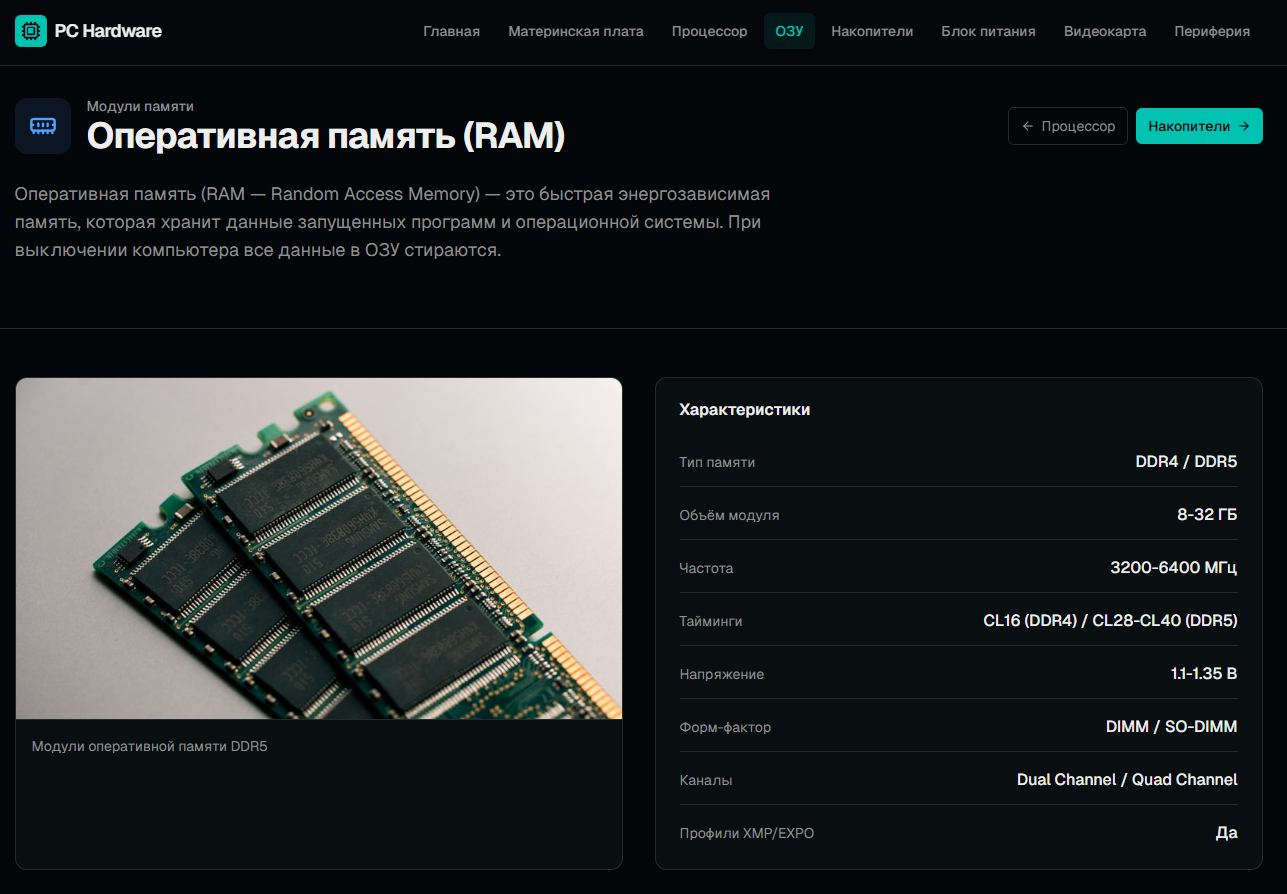
\includegraphics[width=1\linewidth]{screenshots/Снимок экрана 2026-03-12 023616.png}
    \caption{Главная страница}
    \label{fig:placeholder}
\end{figure}

На главной странице (рисунок 1) размещена общая информация о проекте, сведения об учебном заведении и группе, а также сетка карточек с навигацией по всем семи разделам. Каждая карточка содержит иконку, название компонента и краткое описание.

\subsection{Раздел <<Материнская плата>>}

В данном разделе (рисунок~\ref{fig:motherboard}) представлена информация о материнской плате как центральном компоненте, объединяющем все остальные устройства. Описаны форм-факторы (ATX, Micro-ATX, Mini-ITX), типы сокетов (LGA~1700, AM5), чипсеты, слоты расширения и порты подключения. Перечислены основные производители: ASUS, MSI, Gigabyte, ASRock.

\begin{figure}[h!]
    \centering
    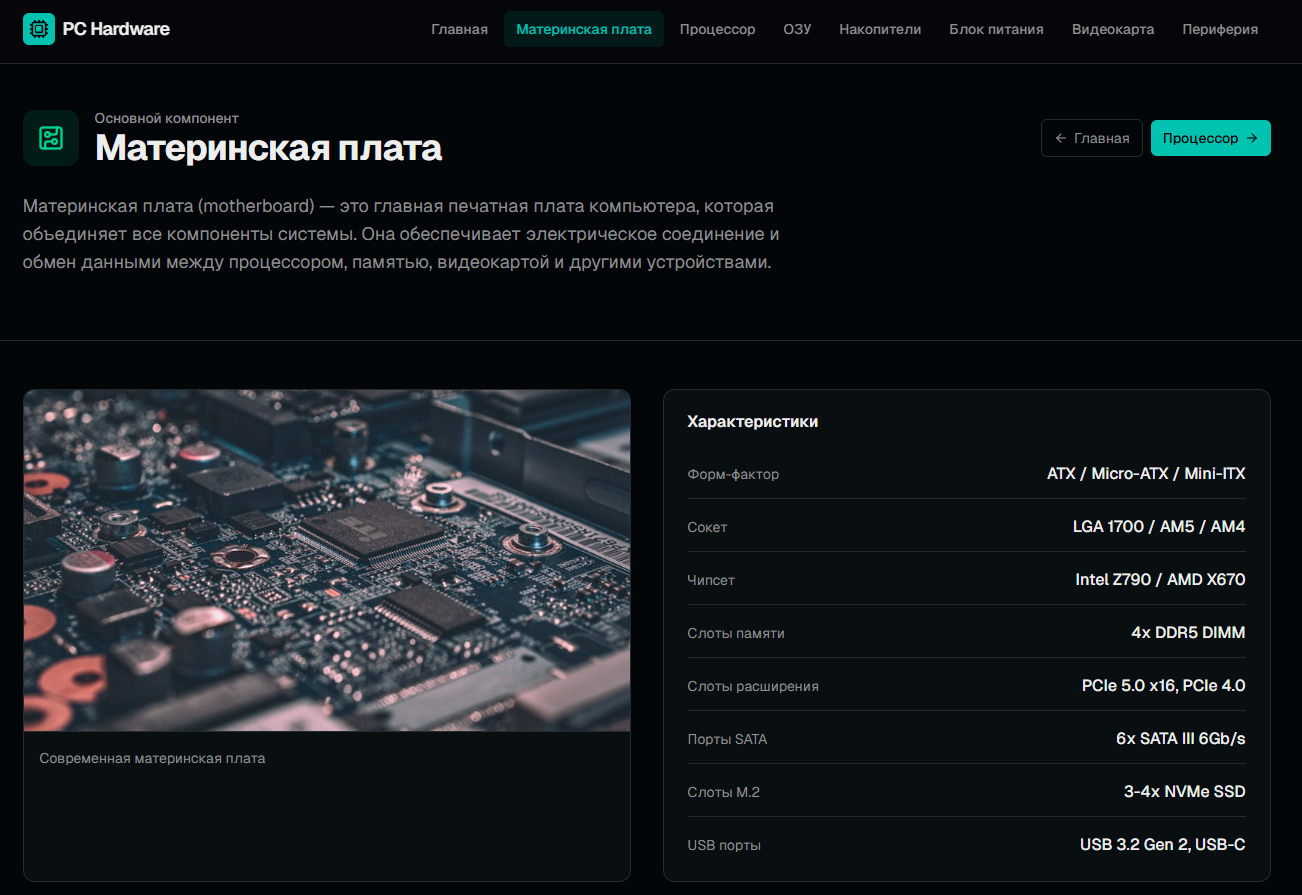
\includegraphics[width=1\linewidth]{screenshots/Снимок экрана 2026-03-12 024722.png}
    \caption{траница раздела <<Материнская плата>>}
    \label{fig:motherboard}
\end{figure}

\subsection{Раздел <<Процессор>>}

Раздел посвящён центральному процессору (рисунок~\ref{fig:cpu}). Приведены характеристики современных процессоров: количество ядер (8--24), тактовая частота (до 6{,}0~ГГц), объём кэш-памяти L3 (32--96~МБ), тепловыделение (65--125~Вт). Описаны технологии многопоточности и рекомендации по выбору процессора в зависимости от задач.

\begin{figure}[h!]
    \centering
    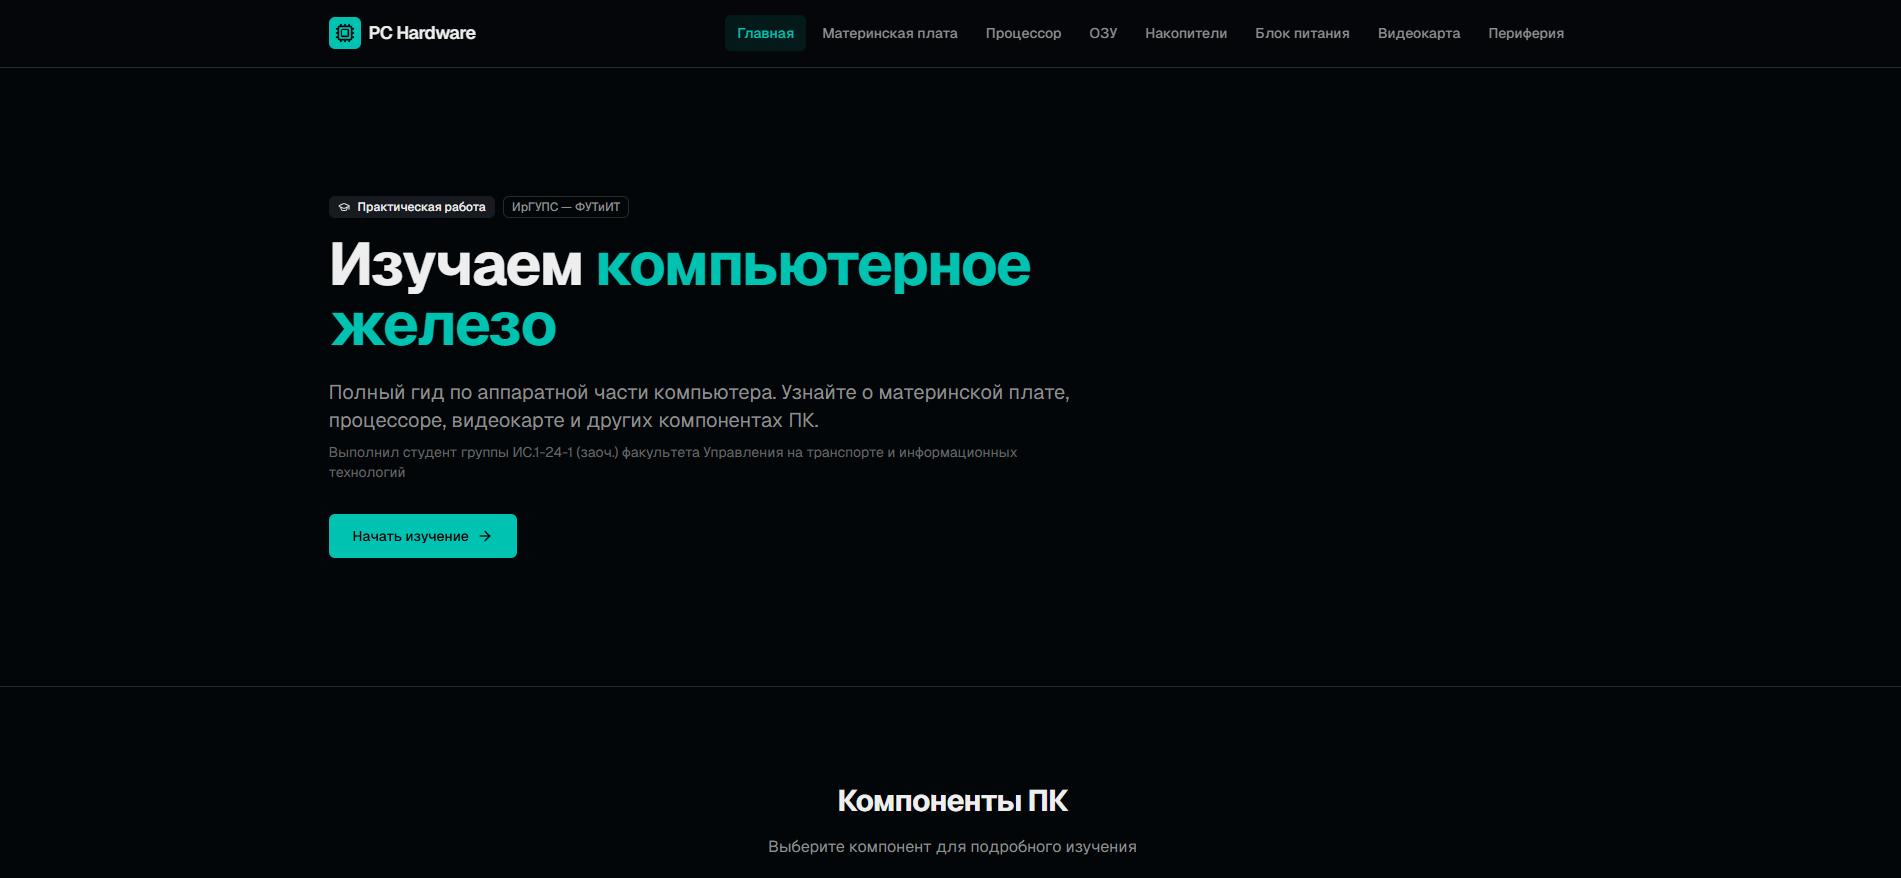
\includegraphics[width=1\linewidth]{screenshots/Снимок экрана 2026-03-12 025020.png}
    \caption{Страница раздела <<Процессор>>}
    \label{fig:cpu}
\end{figure}

\subsection{Раздел <<Оперативная память>>}
\begin{figure}[h!]
    \centering
    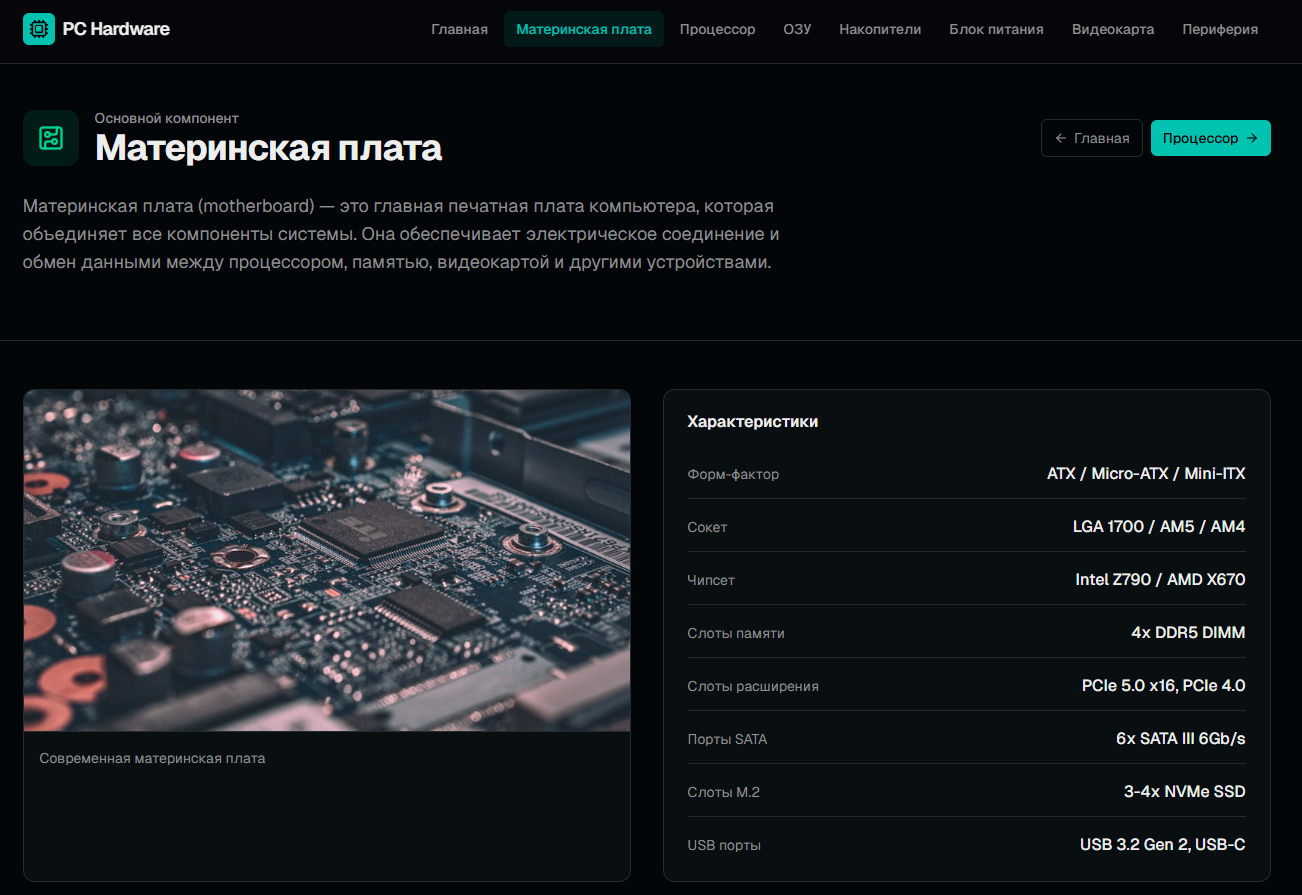
\includegraphics[width=1\linewidth]{screenshots/Снимок экрана 2026-03-12 025139.png}
    \caption{Страница раздела <<Оперативная память>>}
    \label{fig:ram}
\end{figure}
На странице оперативной памяти (рисунок~\ref{fig:ram}) описаны стандарты DDR4 и DDR5, параметры частоты и таймингов, режимы двухканальной работы и профили автоматического разгона XMP/EXPO. Указано, что минимальный рекомендуемый объём для комфортной работы в 2026 году составляет 16~ГБ.


\newpage
\subsection{Раздел <<Накопители>>}

В разделе накопителей (рисунок~\ref{fig:storage}) проведено сравнение HDD и SSD, описаны интерфейсы SATA~III и NVMe (PCIe~4.0/5.0), форм-факторы (2.5\textquotedbl, 3.5\textquotedbl, M.2~2280). Приведены актуальные скоростные характеристики: до 14\,000~МБ/с для чтения NVMe PCIe~5.0.

\newpage
\begin{figure}[h!]
    \centering
    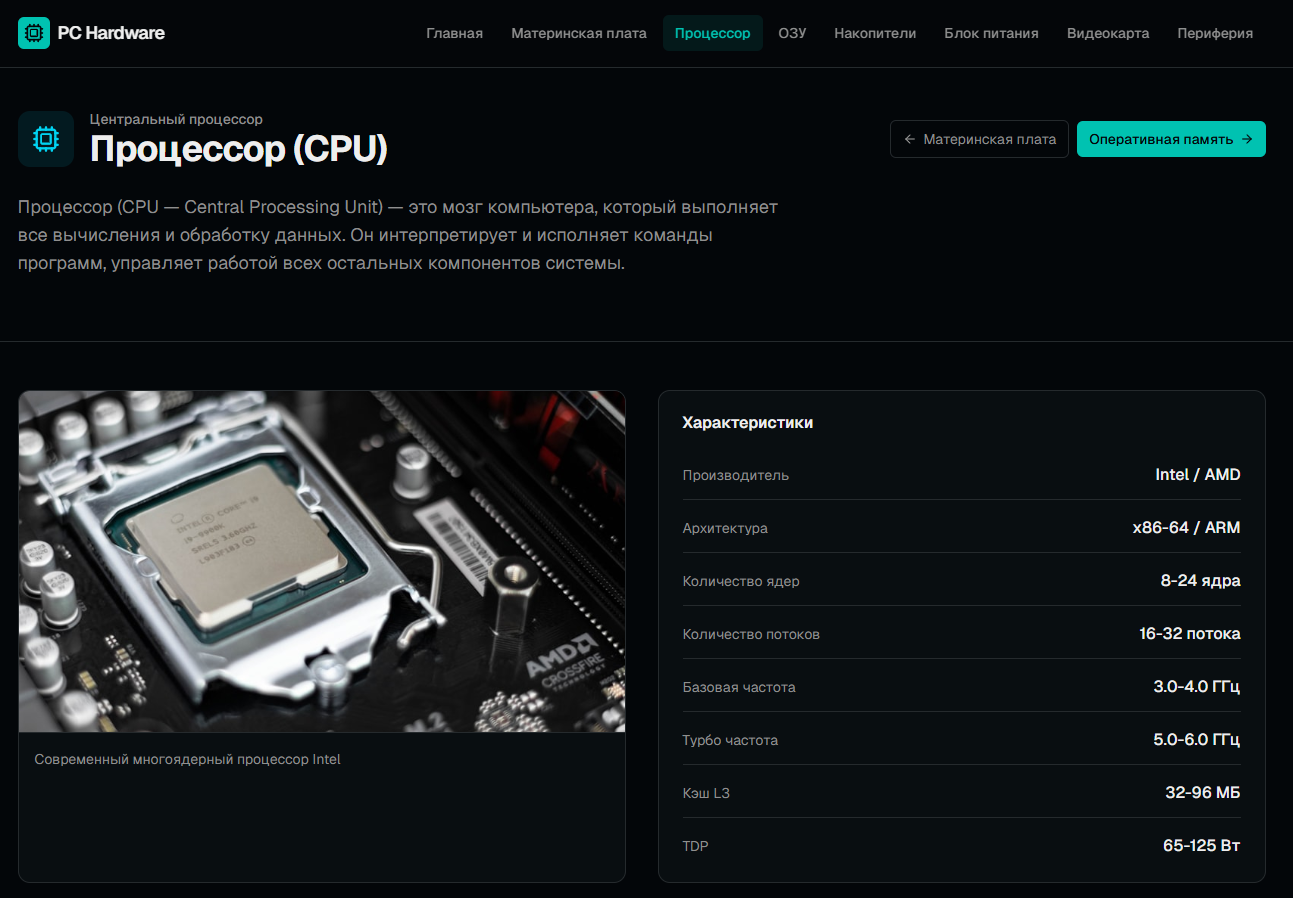
\includegraphics[width=1\linewidth]{screenshots/Снимок экрана 2026-03-12 025517.png}
    \caption{Страница раздела <<Накопители>>}
    \label{fig:storage}
\end{figure}
\subsection{Раздел <<Блок питания>>}

Страница блока питания (рисунок~\ref{fig:psu}) содержит информацию о преобразовании напряжения, сертификации 80~Plus, модульности кабельной системы и системах защиты. Рассмотрены критерии выбора мощности с учётом запаса 20--30\% от расчётного энергопотребления системы.
\newpage
\begin{figure}[h!]
    \centering
    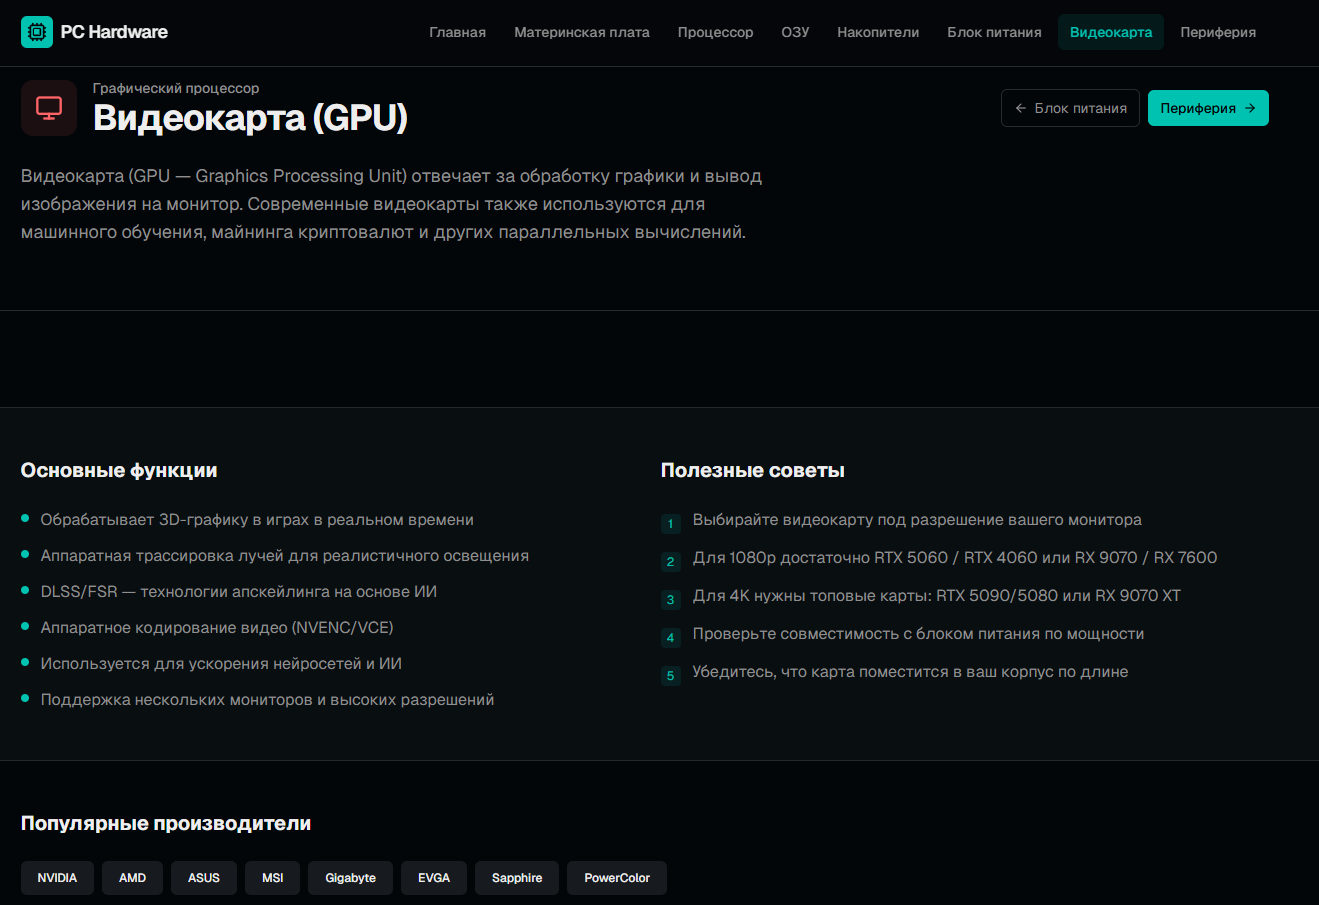
\includegraphics[width=1\linewidth]{screenshots/Снимок экрана 2026-03-12 025806.png}
    \caption{Страница раздела <<Блок питания>>}
    \label{fig:psu}
\end{figure}
\subsection{Раздел <<Видеокарта>>}

В разделе видеокарты (рисунок~\ref{fig:gpu}) описаны ключевые параметры: объём видеопамяти (8--24~ГБ GDDR6X), шина памяти, тактовая частота GPU, количество шейдерных процессоров. Рассмотрены технологии аппаратной трассировки лучей и ИИ-апскейлинга (DLSS, FSR). Приведены рекомендации по выбору видеокарты в зависимости от разрешения монитора.

\newpage
\begin{figure}[h!]
    \centering
    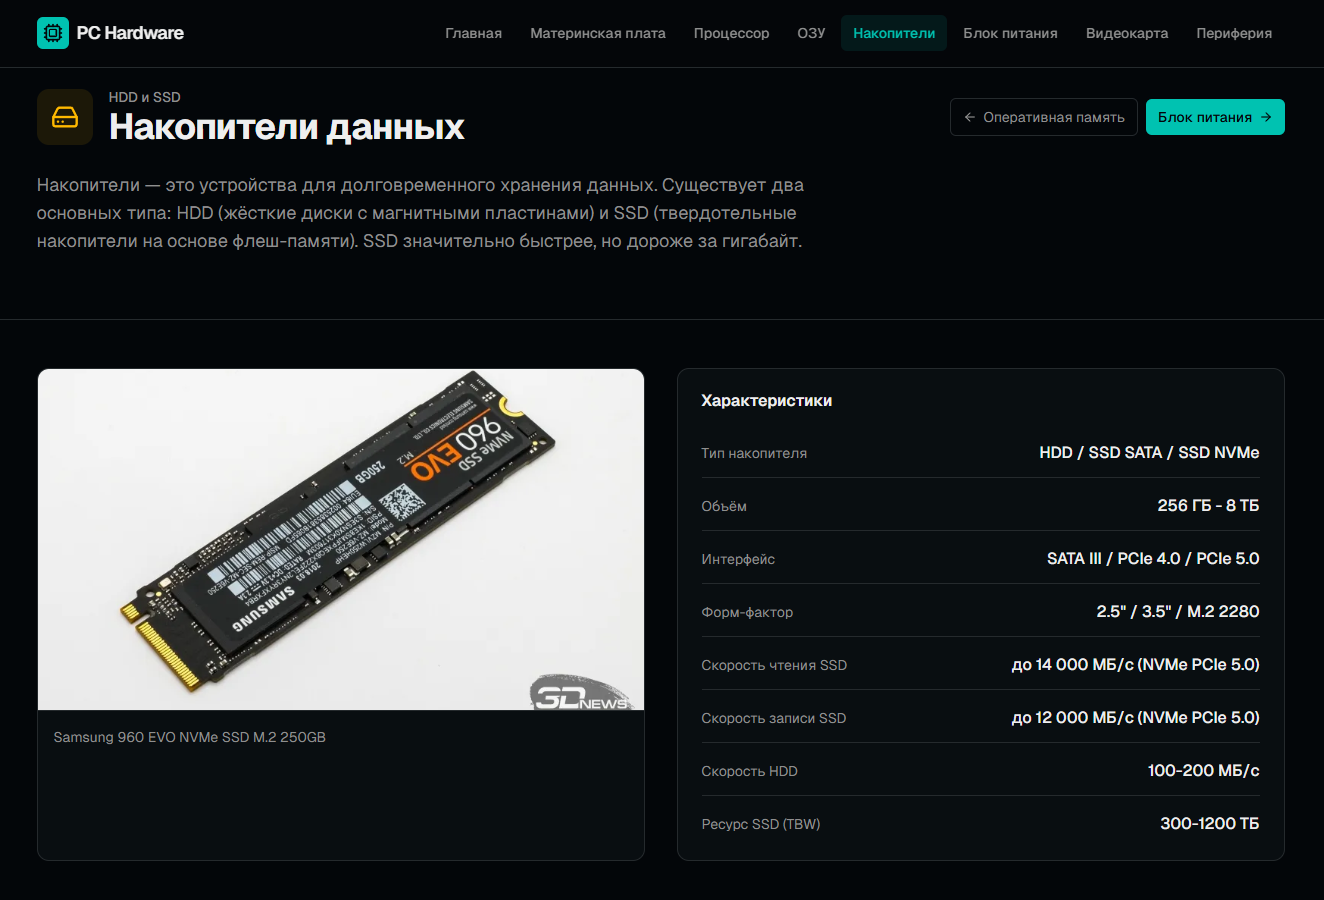
\includegraphics[width=1\linewidth]{screenshots/Снимок экрана 2026-03-12 030224.png}
    \caption{Страница раздела <<Видеокарта>>}
    \label{fig:gpu}
\end{figure}

\subsection{Раздел <<Периферия>>}

Раздел периферийных устройств (рисунок~\ref{fig:peripherals}) является наиболее обширным и охватывает шесть категорий: мониторы, клавиатуры, мыши, аудиоустройства, веб-камеры и игровые контроллеры. Для каждой категории представлены ключевые характеристики, типы устройств и рекомендации по выбору.

\newpage
\begin{figure}[h!]
    \centering
    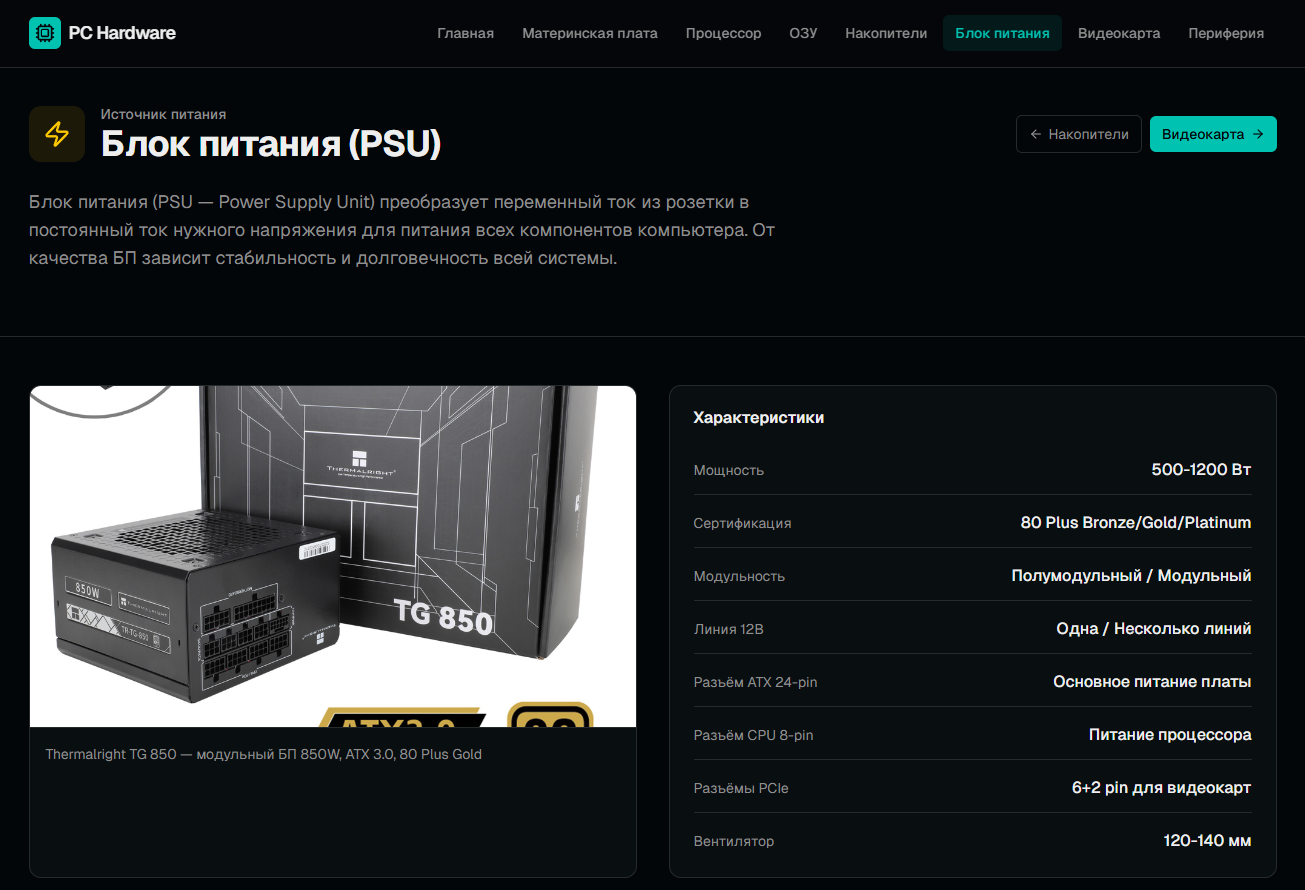
\includegraphics[width=1\linewidth]{screenshots/Снимок экрана 2026-03-12 030408.png}
    \caption{Страница раздела <<Периферия>>}
    \label{fig:peripherals}
\end{figure}

\subsection{Техническая реализация}

Приложение построено с использованием архитектуры App Router фреймворка Next.js. Файловая структура проекта определяет маршрутизацию: каждая папка в директории \texttt{app/} соответствует отдельному URL-маршруту.

Для обеспечения единообразия оформления разделов был разработан переиспользуемый компонент \texttt{ComponentPageLayout}, который принимает набор типизированных свойств (заголовок, описание, характеристики, иллюстрацию, советы, список производителей) и формирует страницу по единому шаблону. Такой подход позволяет централизованно управлять макетом и упрощает добавление новых разделов.

Навигация реализована на двух уровнях. Глобальная навигация представлена фиксированной шапкой с ссылками на все разделы, которая на мобильных устройствах трансформируется в выпадающее меню. Последовательная навигация обеспечивается кнопками <<Назад>> и <<Далее>>, расположенными в верхней и нижней частях каждой страницы.

Адаптивный дизайн реализован по принципу <<Mobile First>> средствами Tailwind~CSS. Сетка карточек на главной странице автоматически перестраивается от одной колонки на мобильных экранах до трёх колонок на десктопных. Цветовая схема построена на цветовом пространстве OKLCh, обеспечивающем перцептуальную равномерность оттенков.

% ===========================================================================
% ЗАКЛЮЧЕНИЕ
% ===========================================================================
\newpage
\section*{ЗАКЛЮЧЕНИЕ}
\addcontentsline{toc}{section}{ЗАКЛЮЧЕНИЕ}

В ходе прохождения учебной (ознакомительной) практики были выполнены все поставленные задачи. Изучен состав и назначение основных аппаратных компонентов персонального компьютера, освоены современные средства веб-разработки, разработано и развёрнуто образовательное веб-приложение, систематизирующее полученные знания.

Результатом практики стало веб-приложение <<PC~Hardware~Guide>>, содержащее восемь страниц с информацией о материнской плате, процессоре, оперативной памяти, накопителях, блоке питания, видеокарте и периферийных устройствах. Каждый раздел включает технические характеристики, описание функций, рекомендации по выбору и перечень производителей. Приложение обеспечивает адаптивное отображение на устройствах с различными размерами экрана и удобную навигацию между разделами.

В процессе выполнения практического задания были применены современные информационные технологии и программные средства для решения задач профессиональной деятельности. Продемонстрировано понимание принципов работы вычислительных систем и их компонентной архитектуры. Освоены методики использования программных средств веб-разработки, включая фреймворк Next.js, язык TypeScript и инструменты стилизации Tailwind~CSS, для решения практической задачи создания образовательного ресурса.

Приложение может быть использовано в качестве справочного материала при изучении аппаратной части вычислительных систем.

% ===========================================================================
% СПИСОК ИСПОЛЬЗОВАННЫХ ИСТОЧНИКОВ
% ===========================================================================
\newpage
\section*{СПИСОК ИСПОЛЬЗОВАННЫХ ИСТОЧНИКОВ}
\addcontentsline{toc}{section}{СПИСОК ИСПОЛЬЗОВАННЫХ ИСТОЧНИКОВ}

\begin{enumerate}
  \item Таненбаум Э., Остин Т. Архитектура компьютера. 6-е изд. СПб.: Питер, 2022. 816~с.
  \item Олифер В.\,Г., Олифер Н.\,А. Компьютерные сети. Принципы, технологии, протоколы. 5-е изд. СПб.: Питер, 2020. 992~с.
  \item Документация Next.js [Электронный ресурс]. --- URL: \url{https://nextjs.org/docs} (дата обращения: 11.03.2026).
  \item Документация React [Электронный ресурс]. --- URL: \url{https://react.dev} (дата обращения: 11.03.2026).
  \item Документация Tailwind CSS [Электронный ресурс]. --- URL: \url{https://tailwindcss.com/docs} (дата обращения: 11.03.2026).
  \item Документация TypeScript [Электронный ресурс]. --- URL: \url{https://www.typescriptlang.org/docs} (дата обращения: 11.03.2026).
  \item Motherboard // Wikipedia [Электронный ресурс]. --- URL: \url{https://en.wikipedia.org/wiki/Motherboard} (дата обращения: 11.03.2026).
  \item Central processing unit // Wikipedia [Электронный ресурс]. --- URL: \url{https://en.wikipedia.org/wiki/Central_processing_unit} (дата обращения: 11.03.2026).
  \item Solid-state drive // Wikipedia [Электронный ресурс]. --- URL: \url{https://en.wikipedia.org/wiki/Solid-state_drive} (дата обращения: 11.03.2026).
  \item Graphics processing unit // Wikipedia [Электронный ресурс]. --- URL: \url{https://en.wikipedia.org/wiki/Graphics_processing_unit} (дата обращения: 11.03.2026).
\end{enumerate}

\end{document}
